\chapter{DESKRIPSI SUB SISTEM}

Karena sistem yang akan dibuat menggunakan desain berorientasi objek, maka penjelasan lebih detail dari sub-sistem ini akan lebih mudah bila kita melihat diagram \textit{class} yang telah dijelaskan dan digambarkan pada bagian sebelumnya, namun kali ini akan dijelaskan lebih detail.

\section{Kelas AppInitializer}

Kelas ini menjadi kelas pembuka bagi sistem aplikasi yang menggunakan \textit{framework} Spring karena kelas ini mengimplementasikan \textit{interface} dari \textit{framework} Spring yang bernama AbstractAnnotationConfigDispatcherServletInitializer.

Diagram dari kelas AppInitializer ini seperti ditunjukkan pada gambar \ref{fig:uml-class-AppInitializer} :

\begin{figure}[H]
  \centering
  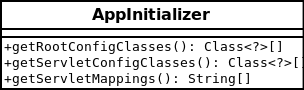
\includegraphics[width=0.5\textwidth]{./resources/uml/uml-class-AppInitializer}
  \caption{Diagram Kelas AppInitializer}
  \label{fig:uml-class-AppInitializer}
\end{figure}

Karena kelas ini adalah implementasi dari \textit{interface} AbstractAnnotationConfigDispatcherServletInitializer, maka harus mengimplementasikan pula ketiga \textit{method} yang ada pada \textit{interface} tersebut, yaitu \textit{method} getRootConfigClasses, \textit{method} getServletConfigClasses, dan \textit{method} getServletMappings.

\section{Kelas AppConfig}

Kelas ini merupakan kelas konfigurasi yang digunakan \textit{framework} Spring untuk melakukan konfigurasi terhadap sistem aplikasi yang akan dijalankan. Bukan karena mengimplementasikan kelas atau \textit{interface} yang dibawa oleh Spring, melainkan karena dideklarasikan sebagai kelas yang menangani konfigurasi sistem aplikasi di kelas AppInitializer.

Pada kelas ini, karena menggunakan fitur MVC (\textit{Model-View-Controller}) dari Spring, maka akan ada beberapa kelas yang ditujukan untuk fungsinya masing-masing, dikelas inilah nantinya kelas-kelas tersebut dideklarasikan, pada kelas ini pula disebutkan kelas yang bertanggung jawab untuk melakukan konfigurasi-konfigurasi yang lain termasuk konfigurasi komunikasi dengan sistem basis data.

Diagram dari kelas AppConfig ini seperti ditampilkan pada gambar \ref{fig:uml-class-AppConfig} :

\begin{figure}[H]
  \centering
  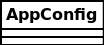
\includegraphics[width=0.3\textwidth]{./resources/uml/uml-class-AppConfig}
  \caption{Diagram Kelas AppConfig}
  \label{fig:uml-class-AppConfig}
\end{figure}

Kelas ini memang terlihat kosong, karena konfigurasi-konfigurasi yang dilakukan nantinya akan menggunakan fitur \textit{annotation} milik Java agar memudahkan pembacaan kode dan menyederhanakan konfigurasi.

\section{Kelas HibernateConfiguration}

Kelas ini bertugas melakukan konfigurasi komunikasi dengan sistem basis data. Diagram dari kelas HibernateConfiguration ini seperti terlihat pada gambar \ref{fig:uml-class-HibernateConfiguration} :

\begin{figure}[H]
  \centering
  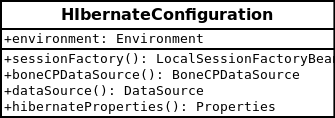
\includegraphics[width=0.8\textwidth]{./resources/uml/uml-class-HibernateConfiguration}
  \caption{Diagram Kelas HibernateConfiguration}
  \label{fig:uml-class-HibernateConfiguration}
\end{figure}

Kelas ini terdiri dari 1 (satu) properti dan 4 (empat) \textit{method}. Propertinya diberi nama environment, karena properti ini akan bertugas menampung nilai-nilai konfigurasi standar yang berada pada \textit{file} yang terpisah.

\textit{Method} yang pertama adalah \textit{method} sessionFactory. \textit{Method} sessionFactory ini akan bertugas mengembalikan nilai sebuah kelas LocalSessionFactoryBean dimana kelas ini yang menjadi sesi dari tiap \textit{user} untuk melakukan koneksi ke basis data nantinya. Untuk menyediakan akses data yang cepat dan optimal, \textit{method} ini akan menggunakan \textit{connection pool} milik BoneCP.

\textit{Method} berikutnya adalah boneCPDataSource, \textit{method} ini akan menyediakan konfigurasi untuk melakukan koneksi ke basis data sebagai sumber data, yang dikembalikan dalam bentuk kelas BoneCPDataSource. \textit{Method} ini menjadi sumber untuk pengambilan data apapun pada basis data dengan menggunakan \textit{connection pool} BoneCP.

\textit{Method} dataSource adalah \textit{method} standar yang menggunakan \textit{connection pool} yang dibawa oleh Hibernate yang digunakan untuk melakukan pemeriksaan awal koneksi ke basis data, apabila menggunakan \textit{method} ini berhasil, maka tidak akan menjadi masalah apabila dilakukan menggunakan \textit{connection pool} yang lain.

\textit{Method} yang terakhir adalah hibernateProperties, \textit{method} ini melakukan konfigurasi terhadap Hibernate yang nantinya digunakan pada \textit{method} sessionFactory.

\section{Kelas SpptRestController}

Kelas ini yang menjadi gerbang pertama yang menentukan kemana sebuah \textit{request} akan di respon. Diagram kelas dari SpptRestController ini akan terlihat seperti pada gambar \ref{fig:uml-class-SpptRestController} :

\begin{figure}[H]
  \centering
  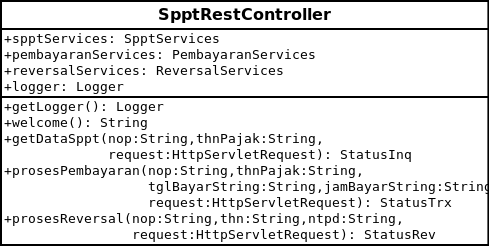
\includegraphics[width=0.8\textwidth]{./resources/uml/uml-class-SpptRestController}
  \caption{Diagram Kelas SpptRestController}
  \label{fig:uml-class-SpptRestController}
\end{figure}

Kelas ini memiliki 4 (empat) properti dan 5 (lima) \textit{method}. Penjelasan dan fungsi masing-masing properti dan \textit{method} tersebut yaitu sebagai berikut :

\begin{itemize}
  \item Properti
  
  \begin{itemize}
    \item Properti spptServices
    
    Properti ini yang akan mengatur layanan yang menangani permintaan / \textit{request inquiry} dari \textit{client}.
    
    \item Properti pembayaranServices
    
    Properti pembayaranServices ini akan mengatur layanan yang menangani permintaan / \textit{request} pencatatan pembayaran dari \textit{client}.
    
    \item Properti reversalServices
    
    Properti reversalServices ini akan mengatur layanan yang menangani permintaan / \textit{request reversal} dari \textit{client} karena ada kesalahan pencatatan pembayaran sebelumnya.
    
    \item Properti logger
    
    Properti logger digunakan untuk melakukan pencatatan aktifitas sistem aplikasi ke dalam sebuah \textit{file} pada saat sistem aplikasi berjalan dan digunakan. Kondisi ini diperlukan agar memudahkan diagnosa sistem apabila terjadi anomali-anomali proses yang tidak diinginkan.
   
  \end{itemize}
  
  \item \textit{Method}
  
  \begin{itemize}
    \item \textit{Method} getLogger
    
    \textit{Method} getLogger ini menyediakan akses ke properti logger agar dapat mencatat kejadian saat \textit{runtime} dari kelas mana pun pada sistem aplikasi.
    
    \item \textit{Method} welcome
    
    \textit{Method} welcome ini adalah halaman muka dari layanan Rest, jadi setiap \textit{request} yang dilayangkan ke \textit{root slash} ("/"), maka akan direspon oleh \textit{method} welcome ini.
    
    \item \textit{Method} getDataSppt
    
    \textit{Method} getDataSppt difungsikan sebagai tempat masuknya \textit{request inquiry} data tagihan SPPT PBB-P2, nantinya \textit{method} ini akan mengembalikan respon dalam bentuk kelas StatusInq yang telah diubah dalam format JSON.
    
    \item \textit{Method} prosesPembayaran
    
    \textit{Method} prosesPembayaran ini akan bertugas menangani \textit{request} pencatatan pembayaran dari \textit{client}. \textit{Method} ini akan mengembalikan kelas StatusTrx yang tentunya telah diubah dalam format JSON.
    
    \item \textit{Method} prosesReversal
    
    \textit{Method} prosesReversal ini seperti \textit{method} getDataSppt dan \textit{method} prosesPembayaran yang menangani sebuah \textit{request} dari \textit{client}, namun \textit{method} prosesReversal ini akan menangani \textit{request reversal} dari pembayaran yang telah tercatat dalam basis data.
    
    Penyebab proses \textit{reversal} ini karena adanya kesalahan pencatatan pembayaran yang sebelumnya terjadi, misalkan pada saat \textit{client} melakukan \textit{request} pencatatan pembayaran, sebelum \textit{client} mendapatkan respon dari \textit{server} koneksi tiba-tiba terputus dan \textit{client} tidak pernah mendapatkan respon atas \textit{request}-nya, maka untuk memastikan adalah melakukan \textit{request reversal} dan melakukan \textit{request} pencatatan pembayaran kembali.
    
  \end{itemize}
\end{itemize}

\section{Kelas SpptServicesImpl}

Kelas SpptServicesImpl akan melayani \textit{request inquiry} dan melanjutkannya ke kelas-kelas yang menangani basis data. Diagram kelas dari SpptServicesImpl ini adalah seperti pada gambar \ref{fig:uml-class-SpptServicesImpl}

\begin{figure}[H]
  \centering
  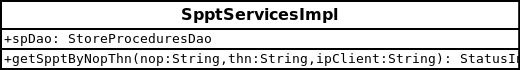
\includegraphics[width=1\textwidth]{./resources/uml/uml-class-SpptServicesImpl}
  \caption{Diagram Kelas SpptServicesImpl}
  \label{fig:uml-class-SpptServicesImpl}
\end{figure}

Kelas SpptServicesImpl ini memiliki 1 (satu) properti dan 1 (satu) \textit{method}. Propertinya bernama spDao, untuk menampung kelas StoreProceduresDao yang menangani semua hal mengenai eksekusi \textit{store procedure} pada basis data.

\textit{Method} dari kelas ini bernama getSpptByNopThn yang berfungsi melakukan pemanggilan terhadap kelas yang bertugas menghubungi basis data yang pencarian datanya berdasarkan Nomor Objek Pajak (NOP) dan tahun pajak.

\section{Kelas PembayaranServicesImpl}

Kelas PembayaranServicesImpl bertugas melayani permintaan terhadap pencatatan pembayaran yang posisinya berada di tengah dan menjadi penghubung antara \textit{interface} dengan kelas-kelas \textit{data access}. Diagram kelas PembayaranServicesImpl ini seperti pada gambar \ref{fig:uml-class-PembayaranServicesImpl} :

\begin{figure}[H]
  \centering
  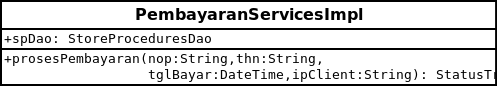
\includegraphics[width=1\textwidth]{./resources/uml/uml-class-PembayaranServicesImpl}
  \caption{Diagram Kelas PembayaranServicesImpl}
  \label{fig:uml-class-PembayaranServicesImpl}
\end{figure}

Kelas ini memiliki 1 (satu) properti dan 1 (satu) \textit{method}, properti yang dimiliki bernama spDao, ini adalah instan dari kelas atau \textit{interface} StoreProceduresDao yang bertugas melakukan komunikasi dengan sistem aplikasi basis data.

Sedangkan \textit{method} prosesPembayaran adalah \textit{method} yang bertugas sebagai penghubung antara \textit{interface} dalam hal ini kelas SpptRestController, dengan kelas yang berhubungan dan berkomunikasi langsung dengan basis data untuk melakukan eksekusi pencatatan pembayaran.

\section{Kelas ReversalServicesImpl}

Seperti kelas PembayaranServicesImpl dan SpptServicesImpl, kelas ReversalServicesImpl bertugas menjadi penghubung antara \textit{interface} yang menangani proses \textit{reversal} dengan kelas-kelas yang berhubungan dengan basis data. 

Diagram kelas ReversalServicesImpl ini seperti terlihat pada gambar \ref{fig:uml-class-ReversalServicesImpl} :

\begin{figure}[H]
  \centering
  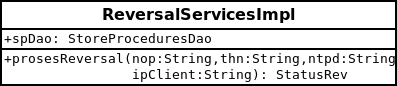
\includegraphics[width=0.5\textwidth]{./resources/uml/uml-class-ReversalServicesImpl}
  \caption{Diagram Kelas ReversalServicesImpl}
  \label{fig:uml-class-ReversalServicesImpl}
\end{figure}

Seperti terlihat pada diagram bahwa kelas ReversalServicesImpl ini memiliki sebuah properti dan sebuah \textit{method}.

Properti yang dimiliki kelas ReversalServicesImpl ini bernama spDao yang merupakan instan dari kelas StoreProceduresDao, dengan \textit{method} bernama prosesReversal, \textit{method} ini nantinya akan berkomunikasi dengan kelas StoreProceduresDao melalui instan kelas spDao yang menjadi penghubung dengan sistem aplikasi basis data.

\section{Kelas StoreProceduresDaoImpl}

Kelas StoreProceduresDaoImpl ini yang mengimplementasikan \textit{interface} StoreProceduresDao yang fungsinya melakukan komunikasi dengan sistem basis data. Diagram kelas StoreProceduresDaoImpl ini seperti terlihat pada gambar \ref{fig:uml-class-StoreProceduresDaoImpl} :

\begin{figure}[H]
  \centering
  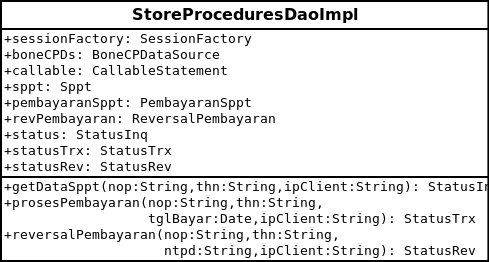
\includegraphics[width=0.8\textwidth]{./resources/uml/uml-class-StoreProceduresDaoImpl}
  \caption{Diagram Kelas StoreProceduresDaoImpl}
  \label{fig:uml-class-StoreProceduresDaoImpl}
\end{figure}

Kelas ini memiliki beberapa properti dan 3 (tiga) buah \textit{method}. Properti yang pertama bernama sessionFactory, ini adalah instan dari kelas SessionFactory yang bertugas membuka sesi komunikasi dengan sistem basis data.

Properti yang kedua adalah boneCPDs, yang merupakan instan dari kelas BoneCPDataSource. Properti ini akan melaksanakan tugasnya dengan \textit{framework} Hibernate menggunakan \textit{connection pool} dari BoneCP untuk hasil komunikasi yang lebih optimal.

Properti yang ketiga adalah callable yang merupakan instan dari kelas CallableStatement, properti ini akan menyediakan perangkat komunikasi yang mampu melakukan eksekusi terhadap \textit{store procedure} yang berada pada basis data.

Properti selanjutnya adalah sppt, pembayaranSppt, dan revPembayaran yang secara berurutan adalah instan dari kelas Sppt, PembayaranSppt, dan ReversalPembayaran. Ketiga properti ini memiliki fungsi yang sama, yaitu menampung nilai yang dikembalikan saat melakukan eksekusi \textit{store procedure} dari sistem basis data.

Properti berikutnya yaitu status, statusTrx, dan statusRev, yang secara berurutan merupakan instan dari kelas StatusInq, StatusTrx, dan StatusRev. Fungsi dari ketiga properti ini yaitu sebagai pembungkus, atau penjelas informasi terhadap respon dari \textit{request} yang dikirimkan oleh \textit{client}.

Untuk \textit{method} yang pertama adalah \textit{method} getDataSppt, yang fungsinya melakukan komunikasi dengan sistem basis data untuk memberikan respon terhadap \textit{request inquiry} dari \textit{client}.

\textit{Method} yang kedua adalah \textit{method} prosesPembayaran, yang fungsinya melakukan komunikasi dengan sistem basis data untuk memberikan respon terhadap \textit{request} pencatatan pembayaran di \textit{client}.

Sedangkan \textit{method} reversalPembayaran berfungsi melakukan komunikasi dengan sistem basis data untuk memberikan respon terhadap \textit{request reversal} pembayaran dari \textit{client}.

\section{Kelas StatusInq}

Kelas StatusInq ini digunakan untuk membungkus data respon sebuah \textit{inquiry} menjadi informasi yang lebih jelas karena ada penjelasan status respon yang diberikan. Misalkan, data \textit{inquiry} tidak muncul, maka kelas ini akan memberikan informasi lain apakah nomor objek pajak yang diminta ada atau tidak, atau kondisi nomor objek pajak tidak muncul karena telah terbayarkan.

Diagram kelas StatusInq ini seperti terlihat pada gambar \ref{fig:uml-class-StatusInq} :

\begin{figure}[H]
  \centering
  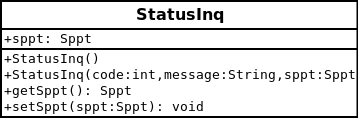
\includegraphics[width=0.5\textwidth]{./resources/uml/uml-class-StatusInq}
  \caption{Diagram Kelas StatusInq}
  \label{fig:uml-class-StatusInq}
\end{figure}

Kelas ini hanya memiliki 1 (satu) properti, 2 (dua) konstruktor, dan 2 (dua) \textit{method}.

Properti pada kelas ini diberi nama sppt yang merupakan instan dari kelas Sppt. Seperti dijelaskan pada bagian sebelumnya, kelas Sppt ini digunakan untuk menampung nilai yang dikembalikan oleh sistem basis data pada saat pemanggilan \textit{store procedure inquiry}.

Kontruktor disediakan 2 (dua), untuk menjadikan kelas ini fleksibel dalam implementasi instan. Sedangkan 2 (dua) \textit{method} yang disediakan sebetulnya untuk melakukan akses \textit{set} dan \textit{get} terhadap properti sppt.

\section{Kelas StatusTrx}

Kelas StatusTrx ini berfungsi membungkus informasi pencatatan transaksi pembayaran agar respon kepada \textit{client} lebih jelas. Diagram kelas dari kelas StatusTrx ini seperti terlihat pada gambar \ref{fig:uml-class-StatusTrx} :

\begin{figure}[H]
  \centering
  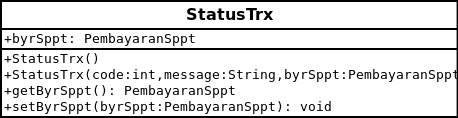
\includegraphics[width=0.5\textwidth]{./resources/uml/uml-class-StatusTrx}
  \caption{Diagram Kelas StatusTrx}
  \label{fig:uml-class-StatusTrx}
\end{figure}

Seperti kelas StatusInq, kelas ini pun memiliki sebuah properti, 2 (dua) buah kontruktor, dan 2 (dua) buah \textit{method}.

Properti pada kelas ini bernama byrSppt yang merupakan instan dari kelas PembayaranSppt, yang fungsinya adalah menampung hasil respon dari sistem basis data atas eksekusi \textit{store procedure} untuk pencatatan pembayaran.

Fungsi dari 2 (dua) kontruktor yang ada pada kelas ini pun ditujukan agar pembentukan instan agar lebih fleksibel. Kedua \textit{method} pun dimaksudkan untuk memberikan akses pada properti dari kelas ini.

\section{Kelas StatusRev}

Kelas StatusRev ini berfungsi untuk membungkus informasi \textit{reversal} agar respon terhadap \textit{request client} lebih jelas. Diagram kelas StatusRev ini dapat dilihat pada gambar \ref{fig:uml-class-StatusRev} :

\begin{figure}[H]
  \centering
  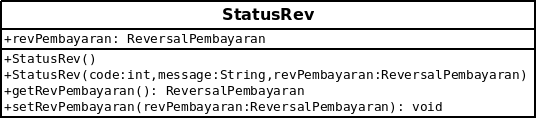
\includegraphics[width=0.8\textwidth]{./resources/uml/uml-class-StatusRev}
  \caption{Diagram Kelas StatusRev}
  \label{fig:uml-class-StatusRev}
\end{figure}

Seperti kelas StatusInq dan StatusTrx, kelas ini pun terdiri dari sebuah properti, 2 (dua) buah konstruktor, dan 2 (dua) buah \textit{method}. 

Properti kelas ini bernama revPembayaran yang merupakan instan dari kelas ReversalPembayaran, yang fungsinya menampung hasil respon dari basis data terhadap eksekusi \textit{store procedure reversal} pembayaran.

Kedua konstruktor yang disediakan untuk menjadikan pembuatan instan kelas ini lebih fleksibel, sedangkan dua \textit{method} yang disediakan merupakan fasilitas untuk melakukan akses terhadap properti kelas ini.

\section{Kelas Sppt}

Kelas Sppt ini adalah kelas yang menampung hasil respon dari pemanggilan atau eksekusi \textit{store procedure inquiry} yang ada pada basis data. Diagram kelas ini seperti terlihat pada gambar \ref{fig:uml-class-Sppt} :

\begin{figure}[H]
  \centering
  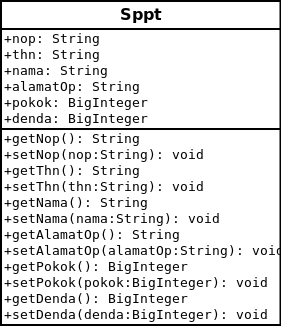
\includegraphics[width=0.5\textwidth]{./resources/uml/uml-class-Sppt}
  \caption{Diagram Kelas Sppt}
  \label{fig:uml-class-Sppt}
\end{figure}

Kelas Sppt ini terdiri dari 6 (enam) properti dan 12 (dua belas) \textit{method}. Enam properti ini adalah nilai-nilai yang dikembalikan dari hasil eksekusi \textit{store procedure} pada basis data. Properti pada kelas ini terdiri dari :

\begin{itemize}
\item nop. Properti ini untuk menyimpan Nomor Objek Pajak, sebagai identitas kunci, tiap objek pajak akan memiliki NOP yang berbeda-beda.
\item thn. Properti ini untuk menampung Tahun Pajak dimana objek pajak dimunculkan tagihan pajaknya.
\item nama. Properti ini akan menampung nama dari wajib pajak untuk nomor objek pajak tersebut pada properti nop.
\item alamatOp. Properti ini untuk menampung alamat dari objek pajak, yang nantinya bisa digunakan sebagai bahan verifikasi bahwa objek tersebut adalah benar yang akan dicari tahu informasinya.
\item pokok. Properti ini untuk menampung besarnya tagihan pokok atas nomor objek pajak yang tersebut pada properti nop.
\item denda. Properti ini akan menampung besarnya denda administrasi yang ditetapkan apabila ada keterlambatan pembayaran pajak yang telah melewati tanggal jatuh temponya.
\end{itemize}

Seluruh \textit{method} yang disediakan pada kelas ini hanya bertujuan untuk melakukan akses terhadap properti pada kelas ini.

\section{Kelas PembayaranSppt}

Kelas PembayaranSppt berfungsi untuk menampung informasi dari respon pencatatan pembayaran SPPT yang terjadi. Diagram kelas dari PembayaranSppt ini seperti terlihat pada gambar \ref{fig:uml-class-PembayaranSppt} :

\begin{figure}[H]
  \centering
  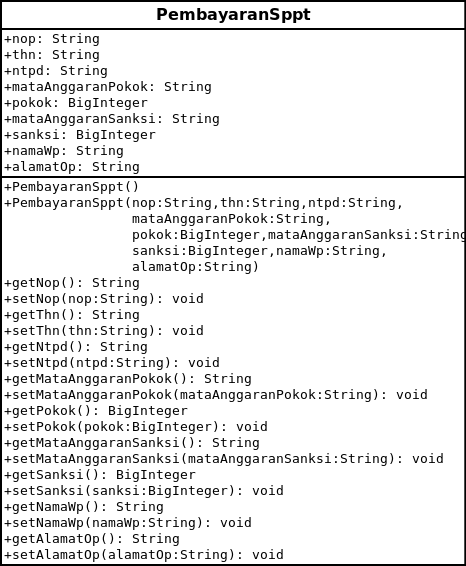
\includegraphics[width=0.5\textwidth]{./resources/uml/uml-class-PembayaranSppt}
  \caption{Diagram Kelas PembayaranSppt}
  \label{fig:uml-class-PembayaranSppt}
\end{figure}

Kelas ini memiliki 9 (sembilan) properti, 2 (dua) kontruktor, dan 18 (delapan belas) \textit{method}. Properti dari kelas ini terdiri dari :

\begin{itemize}
\item nop. Properti nop ini digunakan untuk menampung Nomor Objek Pajak.
\item thn. Properti thn ini digunakan untuk menampung Tahun Pajak dimana NOP dikenakan Pajak Bumi dan Bangunan.
\item ntpd. Properti ntpd ini digunakan untuk menampung Nomor Transaksi Penerimaan Daerah, yang menjadi identitas bahwa pembayaran atas NOP dan Tahun pajak yang diinginkan telah tercatat dalam basis data SISMIOP.
\item mataAnggaranPokok. Properti mataAnggaranPokok ini akan menyimpan kode mata anggaran untuk realisasi penerimaan pokok pajak untuk jenis Pajak Bumi dan Bangunan Perdesaan dan Perkotaan.
\item pokok. Properti pokok ini akan menampung besarnya pokok pajak yang dibayarkan oleh wajib pajak.
\item mataAnggaranSanksi. Properti mataAnggaranSanksi ini akan menampung kode mata anggaran untuk realisasi sanksi administrasi berupa denda dari keterlambatan pembayaran Pajak Bumi dan Bangunan Perdesaan dan Perkotaan.
\item sanksi. Properti sanksi ini akan menampung besarnya denda yang dibayarkan oleh wajib pajak karena keterlambatan pembayaran pokok pajak untuk jenis PBB-P2.
\item namaWp. Properti namaWp ini akan menampung Nama Wajib Pajak yang tercantum dalam SPPT PBB-P2 pada saat terjadinya transaksi pembayaran.
\item alamatOp. Properti alamatOp ini akan menampung Alamat Objek Pajak yang tercantum dalam SPPT-P2 pada saat terjadinya transaksi pembayaran.
\end{itemize}

Dua buah kontruktor yang disediakan seperti pada kelas-kelas sebelumnya, ditujukan untuk fleksibilitas pembentukan instan dari kelas PembayaranSppt ini.

Untuk 18 (delapan belas) \textit{method} yang disediakan, ditujukan untuk keperluan akses properti yang dimiliki oleh kelas PembayaranSppt ini.

\section{Kelas ReversalPembayaran}

Kelas ReversalPembayaran ini berfungsi menampung data-data transaksi \textit{reversal} pembayaran PBB-P2. Diagram kelas ReversalPembayaran ini seperti terlihat pada gambar \ref{fig:uml-class-ReversalPembayaran} :

\begin{figure}[H]
  \centering
  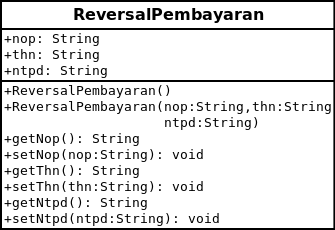
\includegraphics[width=0.5\textwidth]{./resources/uml/uml-class-ReversalPembayaran}
  \caption{Diagram Kelas ReversalPembayaran}
  \label{fig:uml-class-ReversalPembayaran}
\end{figure}

Kelas ini memiliki 3 (tiga) buah properti, 2 (dua) konstruktor, dan 6 (enam) buah \textit{method}.

Properti dari kelas ReversalPembayaran ini terdiri dari :

\begin{itemize}
  \item nop. Properti nop ini berfungsi untuk menampung Nomor Objek Pajak sebagai identitas objek pajak yang akan dilakukan \textit{reversal} pembayarannya.
  \item thn. Properti thn ini berfungsi untuk menampung tahun pajak yang akan dilakukan \textit{reversal} pembayarannya.
  \item ntpd. Properti ntpd ini berfungsi untuk menampung Nomor Transaksi Penerimaan Daerah yang akan dilakukan \textit{reversal} pembayarannya.
\end{itemize}

Dua konstruktor seperti pada kelas-kelas sebelumnya, ditujukan agar pembentukan instan dari kelas ReversalPembayaran ini menjadi lebih fleksibel. Begitu juga dengan 6 (enam) buah \textit{method} yang disediakan kelas ini, difungsikan untuk melakukan akses pada kelas ReversalPembayaran.

Selain kelas-kelas pembentuk aplikasi, di tingkat sistem basis data dibentuk \textit{store procedure}. Daftar \textit{store procedure} yang berada pada basis data adalah sebagai berikut :

\begin{itemize}
  \item SPPT_TERHUTANG. 
  
    \textit{Store procedure} SPPT_TERHUTANG ini nantinya akan mengambil data dari tabel SPPT dan mengembalikan nilainya dalam kolom NOP (Nomor Objek Pajak), THN (Tahun Pajak), NAMA (Nama Wajib Pajak), ALAMAT_OP (Alamat Objek Pajak), POKOK (Besarnya PBB-P2 terhutang), dan DENDA (Besarnya denda administrasi bila ada).

  \item PROSES_PEMBAYARAN. 
  
    \textit{Store procedure} PROSES_PEMBAYARAN ini nantinya akan mengambil data dari tabel SPPT, DAT_OP_BUMI, REF_KELURAHAN, dan REF_KECAMATAN. Keempat tabel tersebut sebagai bahan untuk diformulisikan agar dapat memenuhi pencatatan pada tabel PEMBAYARAN_SPPT yang merupakan tempat mencatatkan pembayaran PBB-P2 yang telah terjadi.
  
    Hasil dari pencatatan pada tabel PEMBAYARAN_SPPT kemudian dijadikan respon pencatatan ke aplikasi yang melakukan eksekusi \textit{store procedure} ini. Keseluruhan transaksi pencatatan tabel PEMBAYARAN_SPPT dan responnya ini kemudian dicatatkan kondisinya pada tabel LOG_TRX_PEMBAYARAN yang memuat NTPD (Nomor Transaksi Penerimaan Daerah).

  \item REVERSAL_PEMBAYARAN.
  
    \textit{Store procedure} REVERSAL_PEMBAYARAN ini nantinya akan mengambil data dari tabel LOG_TRX_PEMBAYARAN, bila ada data pada tabel LOG_TRX_PEMBAYARAN, maka data NOP (Nomor Objek Pajak) untuk Tahun Pajak tersebut pada \textit{request} akan dihapus dari tabel PEMBAYARAN_SPPT, dan mengubah isi kolom STATUS_PEMBAYARAN_SPPT pada tabel SPPT menjadi 0 (karakter nol).
    
    Keseluruhan proses transaksi \textit{reversal} ini dicatat pada tabel LOG_REVERSAL.
\end{itemize}